\chapter{\uppercase{Integrasi SpeaCal dalam RESTU}}
\label{chap:integrasi}

\section{Iterasi III: Desain}

\subsubsection{Perangkat Lunak}

Subsistem penentuan posisi pengguna berdasarkan sinyal suara yang telah didesain pada \autoref{chap:perancangan} harus diintegrasikan dengan RESTU. Pada dasarnya, proses integrasi hanya mencakup proses pengiriman data hasil penentuan posisi yang dihasilkan oleh SpeaCal ke salah satu bagian dari RESTU, misalnya \textit{AI Engine} atau \textit{GUI Engine} (\autoref{fig:speacal_block_diagram}).

Pada konsep \textit{artificial general intelligence} (AGI), semua informasi yang diterima oleh agen, termasuk informasi posisi pengguna, seharusnya masuk ke \textit{AI Engine} terlebih dahulu. Oleh karena bagian kognitif dari RESTU belum menggunakan konsep AGI ini, untuk sementara informasi yang diterima oleh agen diteruskan ke bagian yang langsung membutuhkannya. Dengan demikian, informasi dari subsistem penentuan posisi pengguna berdasarkan sinyal suara dan subsistem penentuan posisi pengguna berdasarkan citra langsung dikirimkan ke \textit{GUI Engine}, tanpa melalui \textit{AI Engine} (\autoref{fig:speacal_block_diagram_rev}). Oleh karena itu, desain pengiriman data dari subsistem penentuan posisi pengguna berdasarkan sinyal suara perlu memperhatikan desain masukan data yang digunakan oleh \textit{GUI Engine}.

\begin{figure}[ht!]
\vskip 1em
\centering
 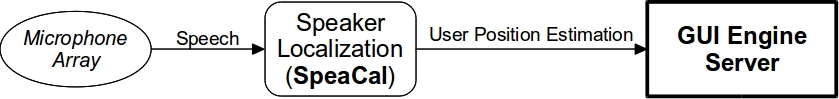
\includegraphics[width=.9\textwidth,keepaspectratio=true]{images/speacal_block_diagram_rev.jpg}
 \caption[Diagram aliran data dari SpeaCal ke \textit{GUI Engine}]{Diagram aliran data dari SpeaCal ke \textit{GUI Engine}.}
 \label{fig:speacal_block_diagram_rev}
\vskip .5em
\end{figure}

\textit{GUI Engine} akan membuka sebuah \textit{socket} untuk pengiriman data dari subsistem penentuan posisi pengguna berdasarkan sinyal suara dan subsistem penentuan posisi pengguna berdasarkan citra. Format penulisan informasi posisi dari dua subsistem tersebut dibedakan agar \textit{GUI Engine} mengetahui darimana informasi berasal. Informasi posisi kemudian dituliskan dalam format koordinat Cartesian tiga dimensi dengan urutan penulisan: koordinat $z$, $y$, kemudian $x$. (\autoref{lst:format_audio}).

\singlespacing
\begin{figure}[htp!]
\vskip 1em
\begin{lstlisting}
a|-30|120|10|
\end{lstlisting}
\caption[Contoh penulisan informasi posisi yang dikirim dari SpeaCal ke \textit{GUI Engine Server}]{Contoh penulisan informasi posisi yang dikirim dari SpeaCal ke \textit{GUI Engine Server}.}
\label{lst:format_audio}
\vskip .5em
\end{figure}
\onehalfspacing

Daerah cakupan subsistem penentuan posisi pengguna berdasarkan citra relatif sempit. Apabila mengacu pada pembagian kawasan yang digunakan oleh subsistem penentuan posisi pengguna berdasarkan sinyal suara (\autoref{fig:floor_plan_2}), subsistem penentuan posisi pengguna berdasarkan citra hanya mencakup kawasan 0 saja.

Prioritas penggunaan informasi posisi pengguna yang berdasarkan citra lebih tinggi daripada informasi yang berdasarkan sinyal suara. Hal ini dikarenakan penentuan posisi pengguna berdasarkan citra menghasilkan posisi yang lebih akurat daripada penentuan posisi berdasarkan sinyal suara. Apabila subsistem penentuan posisi pengguna berdasarkan citra menangkap posisi pengguna melalui dua \textit{webcam} yang digunakannya, \textit{GUI Engine} akan menggunakan informasi posisi dari subsistem tersebut. Apabila tidak ada informasi dari subsistem penentuan posisi berdasarkan citra, \textit{GUI Engine} akan menggunakan informasi dari subsistem penentuan posisi berdasarkan sinyal suara.

Untuk meningkatkan akurasi dalam penentuan posisi pengguna, SpeaCal melakukan tiga kali proses penentuan posisi dengan JST. Hasil dari tiga proses tersebut kemudian diurutkan untuk mencari nilai mediannya. Dengan demikian, apabila sampel sinyal suara yang digunakan untuk menentukan posisi diset $\dfrac{1}{2}$ detik, informasi posisi pengguna akan diperbarui setiap 3 detik.

Informasi posisi yang diterima oleh \textit{GUI Engine} menggunakan format koordinat Cartesian tiga dimensi. Oleh karena itu, nilai median yang diperoleh sebelumnya perlu dikonversi terlebih dahulu dari format kawasan ke format koordinat Cartesian tiga dimensi. Dalam proses konversi koordinat yang dipilih untuk merepresentasikan kawasan adalah koordinat yang terletak pada $y = 120$. Dengan kata lain, $posisi_{kawasan} = {-2, -1, 0, 1, 2}$ dikonversi menjadi $posisi_{Cartesian} = (x, 120, -30)$, dengan $x = {-50, 10, 70, 130, 190}$. Koordinat Cartesian inilah yang kemudian dikirimkan ke \textit{GUI Engine} dengan format seperti yang tercantum pada \autoref{lst:format_audio}.


%%%%%%%%%%%%%%%%%%%%%%%%%%%%%%%%%%%%%%%%%%%

\section{Iterasi III: Implementasi}

\subsubsection{Perangkat Lunak}

Implementasi konversi koordinat dari format kawasan ke format koordinat Cartesian tiga dimensi tertulis pada \autoref{lst:konversi}. Sedangkan, implementasi penyusunan data yang akan dikirimkan ke \textit{GUI Engine} sesuai format penulisan yang telah didefinisikan dan pengiriman data melalui \textit{socket} tertulis pada \autoref{lst:socket}. Dua operasi terkait \textit{socket} tersebut diimplementasikan memanfaatkan pustaka Boost.

\singlespacing
\begin{figure}[htp!]
\vskip 1em
\begin{lstlisting}
speakerPosValue[0] = annResult * 60 + 70;
speakerPosValue[1] = 120;
speakerPosValue[2] = -30;
\end{lstlisting}
\caption[Kode program operasi konversi koordinat]{Kode program operasi konversi koordinat.}
\label{lst:konversi}
\vskip .5em
\end{figure}
\onehalfspacing

\singlespacing
\begin{figure}[htp!]
\vskip 1em
\begin{lstlisting}
try
{
	boost::asio::io_service io_service;
	boost::asio::ip::tcp::resolver resolver(io_service);
	boost::asio::ip::tcp::resolver::query query(boost::asio::ip::tcp::v4(), "167.205.56.139", "12137");
	boost::asio::ip::tcp::resolver::iterator endpoint_iterator = resolver.resolve(query);
	boost::asio::ip::tcp::resolver::iterator end;
	boost::asio::ip::tcp::socket socket(io_service);
	boost::system::error_code error = boost::asio::error::host_not_found;
	while (error && endpoint_iterator != end)
	{
		socket.close();
		socket.connect(*endpoint_iterator++, error);
	}
	if (error)
		throw boost::system::system_error(error);

	std::string pos_info;
	std::string pos_data_start ("a");
	std::string pos_data_separator ("|");

	pos_info.clear();
	pos_info = pos_data_start;
	pos_info += pos_data_separator;
	pos_info += boost::lexical_cast<std::string>(speakerPosValue[2]);
	pos_info += pos_data_separator;
	pos_info += boost::lexical_cast<std::string>(speakerPosValue[1]);
	pos_info += pos_data_separator;
	pos_info += boost::lexical_cast<std::string>(speakerPosValue[0]);
	pos_info += pos_data_separator;

	try
	{
		boost::asio::write(socket, boost::asio::buffer( pos_info ));
		std::cout << pos_info << std::endl;
	}
	catch( std::exception e )
		throw std::runtime_error("message send error | " + std::string( e.what() ) );
}
catch (std::exception& e)
	std::cerr << e.what() << std::endl;
\end{lstlisting}
\caption[Kode program operasi pengiriman data dari SpeaCal ke \textit{GUI Engine} melalui \textit{socket}]{Kode program operasi pengiriman data dari SpeaCal ke \textit{GUI Engine} melalui \textit{socket}.}
\label{lst:socket}
\vskip .5em
\end{figure}
\onehalfspacing

%%%%%%%%%%%%%%%%%%%%%%%%%%%%%%%%%%%%%%%%%%%

\section{Iterasi III: Pengujian dan Evaluasi}

Pengujian menunjukkan bahwa data dari SpeaCal dapat diterima dengan baik oleh \textit{GUI Engine}. Pada saat pengujian, koneksi beberapa kali terputus karena sinyal WLAN yang lemah. Selain itu, tidak ada permasalahan yang dihadapi oleh komunikasi data antara SpeaCal dan \textit{GUI Engine}.

Setelah SpeaCal berhasil diintegrasikan dalam RESTU, pengujian pengguna secara terbatas juga dilakukan. Pengujian melibatkan pihak-pihak yang juga terlibat dalam pengembangan RESTU. Dari proses pengujian, diketahui bahwa SpeaCal dapat menghasilkan informasi posisi pengguna berdasarkan suara pengguna. Meskipun demikian, informasi posisi yang dihasilkan seringkali masih tidak akurat. Dari hasil pengamatan, hasil SpeaCal cenderung berkisar pada nilai -1, 0, dan 1, meskipun pada faktanya pengguna berada pada kawasan -2 atau 2. SpeaCal akan menghasilkan nilai -2 atau 2 apabila jarak pengguna relatif sangat dekat dengan salah satu pasangan mikrofon.

Pengujian menunjukkan bahwa SpeaCal menghasilkan perkiraan posisi yang lebih akurat apabila pengguna memperbesar amplitudo suaranya dengan sedikit berteriak. Selain itu, SpeaCal sensitif terhadap suara yang bersifat \textit{spike}, misalnya suara tepukan tangan dan suara jentikan jari.

Pengujian juga menunjukkan bahwa SpeaCal sangat sensitif terhadap derau. Pada awal pengujian, sebuah \textit{server} diletakkan di samping perangkat \textit{multitouch}, di bawah mikrofon 1-2. Dalam kondisi ini, SpeaCal memiliki kecenderungan menunjukkan nilai -1, bahkan saat tidak ada suara yang dominan di ruangan. Ketika posisi \textit{server} sedikit dimundurkan, kecenderungan menunjukkan nilai -1 berkurang dan SpeaCal kembali menunjukkan nilai 0 saat tidak ada suara pengguna.



%%%%%%%%%%%%%%%%%%%%%%%%%%%%%%%%%%%%%%%%%%%

\section{Analisis Hasil}

Dari proses perancangan lanjutan yang telah dilakukan, beberapa tambahan pencapaian yang telah diperoleh antara lain sebagai berikut.

\begin{enumerate}
\item Menggunakan JST untuk menghasilkan informasi perkiraan posisi pengguna (sumber suara) secara \textit{real-time}, meskipun hasilnya seringkali masih tidak akurat.
\item Mengirimkan informasi perkiraan posisi pengguna ke bagian \textit{GUI Engine} dari RESTU yang kemudian dimanfaatkan untuk menentukan ke arah mana agen virtual menengokkan kepalanya.
\end{enumerate}

Hasil penentuan posisi yang seringkali tidak akurat mungkin disebabkan oleh sensitivitas mikrofon yang kurang memadai. Hal ini ditandai oleh penentuan posisi sering menunjukkan hasil yang akurat apabila penguji (pengguna) mengeluarkan suara yang beramplitudo yang lebih besar dibandingkan dengan saat berbicara normal.

Kurang akuratnya penentuan posisi berdasarkan sinyal suara juga dipengaruhi oleh derau suara yang ada saat penggunaan. Saat sebuah komputer salah satu \textit{server} RESTU diletakkan di bawah mikrofon 1-2, hasil penentuan posisi cenderung menunjukkan nilai -1. Bahkan, dalam kondisi tidak ada pengguna yang bersuara, SpeaCal menunjukkan nilai -1. Hal ini menunjukkan bahwa suara kipas dari komputer tersebut menjadi derau bagi SpeaCal. Dengan demikian, mengganti mikrofon dengan yang lebih baik pun tidak cukup untuk meningkatkan akurasi SpeaCal karena dengan mikrofon yang lebih sensitif berarti semakin banyak pula derau yang tertangkap.

Alternatif solusi yang lain adalah menambahkan operasi pra-pemrosesan sinyal. Sebagai contoh, penggunaan \textit{filter} dimungkinkan untuk memperkecil pengaruh derau yang potensial ada di lingkungan penggunaan RESTU, misalnya derau kipas komputer. Sebenarnya SpeaCal telah mengimplementasikan \textit{biquad band-pass filter} untuk jangkauan frekuensi 300-3300 Hz yang merupakan jangkauan frekuensi suara manusia. Akan tetapi, tampaknya penggunaan \textit{filter} tersebut saja tidak cukup untuk menghasilkan penentuan posisi pengguna yang baik.

Salah satu batasan masalah dalam penelitian ini adalah hanya ada satu sumber suara (pengguna). Di luar batasan tersebut, potensi derau yang terbesar dari SpeaCal adalah suara manusia yang statusnya bukan pengguna. Alternatif solusi dari permasalahan ini adalah pengembangan subsistem penentuan posisi pengguna berdasarkan audiovisual yang mengintegrasikan proses penentuan posisi berdasarkan sinyal suara dan citra, tidak hanya mengombinasikan hasil dari dua proses penentuan posisi berdasarkan sinyal suara dan citra yang terpisah.
